\lab{Application}{Six Degrees of Kevin Bacon}{Six Degrees of Kevin Bacon}
\label{lab:SixDegreesKevinBacon}
\objective{This section uses the parlor game the Six Degrees of Kevin Bacon as an application to graphs}

\section*{Shortest Path Algorithms for Unweighted Graph}
Let $A$ be a unweighted graph. We want to find the shortest path between to nodes. One way we can calculate this is we can do a breath first search and stop when reach the target node. The downside to doing it this way is that the algorithm will look through every node on any level before we reach the target node. Let us pretend that for two nodes $a, b \in A$ that the distance between $a$ and $b$ is 5. Also supose that going from $a$to $b$ you have to check $2^n$ elements where $n$ in the level. So 2 nodes are one away from $a$ four nodes are 2 away from $a$ and so on. You would have to check at least 32 nodes before you would get to $b$.

A better way to find the shortest path is to do a breath first search from both $a$ and $b$. So you calculate all the nodes one away from $a$ and then all the nodes one away from $b$, then two away from $a$, then two away from $b$ and so on until you find a node that is connected to $a$ and $b$. If you assume there is also $2^n$ at the nth level away from $b$ then the number of nodes you have to check before reaching the shortest path is only at least 12 and at most 20.

When you have much more nodes each level away the speed up from doing a breath first search from both sides is much greater. This is one of the best way to find shortest paths in unwieghted undirected graphs. For weighted graphs there are many algorthms that find the shortest path. Those interested should look at Dijkstra's algorithm, Bellman–Ford algorithm, A* search algorithm, Floyd–Warshall, and Johnson's algorithm.


\begin{figure}[h]
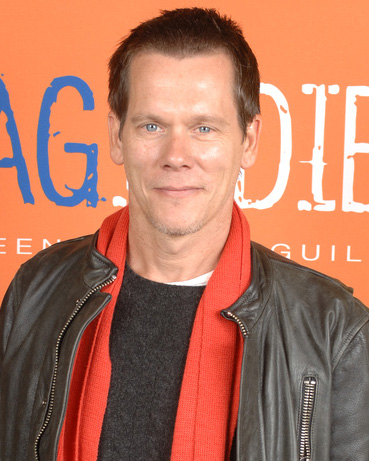
\includegraphics[scale = .4]{Kevin_Bacon.jpg}
\caption{Kevin Bacon.  Image source: Wikipedia.}
\end{figure}

\section*{Six Degrees of Kevin Bacon}
\begin{figure}[h]
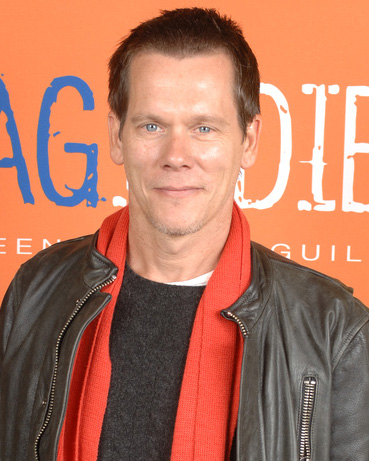
\includegraphics[scale = .4]{Kevin_Bacon.jpg}
\caption{Kevin Bacon.  Image source: Wikipedia.}
\end{figure}

Kevin Bacon is a famous actor who has been in a lot of movies. The six degrees of Kevin Bacon came from a comment made in an interview where Bacon said that he had worked with everyone in Hollywood or someone who's worked with them.  The idea is that you can connect actors to Kevin Bacon. Each actor has a Bacon number that is found as follows:
\begin{enumerate}
\item Kevin Bacon has a Bacon number of 0
\item Actors that have been in a movie with Kevin Bacon have a Bacon number of 1
\item For all other actors $X$, if the lowest number of any actor that $X$ has been in a film with is $n$, $X$ has a Bacon number of $n+1$
\end{enumerate}

\begin{figure}[h]
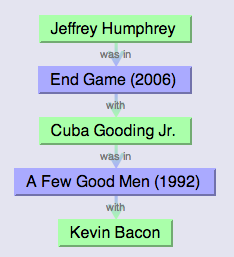
\includegraphics[scale = .6]{Example}
\caption{Jeffery Humphery was in End Game with Cuba Gooding Jr. who was in A Few Good Men with Kevin Bacon, so Jeffrey Humphrey has a Bacon Number of 2.  Image source: http://oracleofbacon.org/.}
\end{figure}

You can define a graph in the same way where each actor is a node and there is an edge between any two nodes if the actors were in a movie together. From this you can find the shortest path between any actor and Kevin Bacon. Of course this can be done with any actor and just not Kevin Bacon. There are equivalents in other fields, the most famous being the Erdos numbers, how far away you are to publishing a paper with the prolific mathematician with Paul Erdos.

\section*{Shortest Paths}
A breath first search can be used to find the shortest path between two nodes of a graph.  However, in practice, breadth first searches are slow for large graphs. Two other algorithms that are often used are Djikstra's algorithm and A*. For this lab, we are going to use a network library called NetworkX. NetworkX allows us to create and manipulate large, complex networks.  Since NetworkX uses Python objects to represent its graphs internally, graphs with lots of nodes will take a large chunk of memory.  Other network libraries exist which are written C++, like igraph, which may significantly reduce the overhead of storing the graph.
To make an undirected graph in NetworkX you do the following:
\begin{lstlisting}
import networkx as nx
G = nx.Graph()
\end{lstlisting}
You to add nodes you use the \li{add_node(x)} method where $x$ is the node you want to add.  If you add an edge between two non-existent nodes, they missing nodes will also be added to the graph. Adding an edge is done by the \li{add_edge(x,y)} method where $x$ and $y$ are previously added nodes. You can add multiple edges or nodes with the methods \li{add_edges_from()} and \li{add_nodes_from()} methods respectively.  There are also \li{has_node(x)} and \li{has_edge(x,y)} that tell you if the node or edge is already added.
\begin{lstlisting}
G.add_node(x)
G.add_edge(x, y)
\end{lstlisting}

\begin{problem}
The data file, \texttt{movieData.txt}, contains the entire casts movies made from 2011 to August of 2013. The file is a delimted file with each field delimited by the '/' character.
Write a method that will open the file, generate a NetworkX graph, and return the constructed graph.
For later solutions, it might be beneficial to also construct a lookup table that maps actors to the movies that they appeared in.
\end{problem}

The \li{shortest_path(G, x, y)} function in NetworkX outputs a list that is one of the shortest paths between $x$ and $y$ in graph $G$.  In an unweighted graph, it finds the shortest path using a pair of breadth first searches originating at the two target nodes.  It advances each breadth first search until they meet and then  constructs the shortest path of nodes.  If no target is specified, the function will find the shortest paths between $x$ and every other node in the network.  It will return the results in a dictionary.  If more than one ``shortest path'' exists, it will return the first one it finds.  We can find the length of the shortest path using the \li{shortest_path_length(G, x, y)} function.

\begin{problem}
Find the shortest path between Kevin Bacon and Liam Neeson. Then find the shortest path from Kevin Bacon to Imran Zahid. Write a function that will accept a path and output the path with the movies in between that connect the actors. Output the paths from Kevin Bacon to Liam Neeson and Imran Zahid with the connecting movies.
\end{problem}

\begin{problem}
Find the average Bacon number for the dataset. Then find how many people have each Bacon number and how many people are not connected to Kevin Bacon (these people have a Bacon number of infinity).
\end{problem}

